\documentclass[12pt, a4paper]{article}
\usepackage[T1]{fontenc}
\usepackage{lmodern}
\usepackage[portuguese]{babel}
\usepackage{graphicx}
\usepackage{geometry}
\usepackage{amsmath}
\usepackage{booktabs} % For better-looking tables
\usepackage{siunitx} % For proper number formatting
\usepackage{float} % For controlling figure placement

\geometry{
 a4paper,
 left=3cm,
 top=2cm,
 right=2cm,
 bottom=2cm
}

\begin{document}

\begin{center}
    \textbf{\large UNIVERSIDADE FEDERAL DO RIO GRANDE DO SUL} \\
    \textbf{\large INSTITUTO DE FÍSICA} \\
    \vspace{3cm}
    \textbf{\Large CADERNO DE LABORATÓRIO 2} \\
    \vspace{1cm}
    \textbf{\large DETERMINAÇÃO DA CONSTANTE DE TEMPO DO CIRCUITO RC} \\
    \vspace{3cm}
    
    \begin{tabular}{rl}
        \textbf{Integrantes:} & Guilherme Franke Riter - 00579589 \\
                               & Júlia Matzenbacher Henicka Germano - 00579271 \\
                               & Leonardo Kawai Suarez - 00578511 \\
                               & Leonardo Werner Morel Dias - 00590887 \\
    \end{tabular}
    
    \vspace{12cm}
    \textbf{\large Porto Alegre, RS} \\
    \textbf{\large 14 de maio de 2025} \\
\end{center}\newpage

\subsection*{Parte A: Montagem e avaliação do comportamento do circuito}
    Podemos calcular a constante de tempo \(\tau\) do circuito RC por três caminhos.
    \begin{itemize}
        \item [(i)] Valores nominais de \(R\) e \(C\)
            \begin{itemize}
                \item [(a)] \(R_n^1 = 5.6 \, \text{k}\Omega\)
                \item [(b)] \(C_n = 47 \, \text{nF}\)
                \item [(c)] \(\tau_n = R_n^1 \cdot C_n = 5.6 \, \text{k}\Omega \cdot 47 \, \text{nF} = 0.2632 \, \text{ms}\)
            \end{itemize}
        \item [(ii)] Valores medidos de \(R\) e \(C\)
            \begin{itemize}
                \item [(a)] \(R_m^1 = 5.57 \, \text{k}\Omega\)
                \item [(b)] \(R_m^2 = 5.54 \, \text{k}\Omega\)
                \item [(c)] \(C_m = 50.9 \, \text{nF}\)
                \item [(d)] \(\tau_m = R_m^1 \cdot C_m = 5.57 \, \text{k}\Omega \cdot 50.9 \, \text{nF} = 0.2834 \, \text{ms}\)
            \end{itemize}
        \item [(iii)] Estimativa visual a partir do osciloscópio
                
            Com \(R_m^1 = 5.57 \, \text{k}\Omega\) e \(C_m = 50.9 \, \text{nF}\), o tempo decorrido \(\tau\) para a tensão cair para aproximadamente \(36.8\% \) do valor inicial é \(\approx 300\mu\text{s}\).
    \end{itemize}

\subsection*{Parte B: Avaliação qualitativa dos efeitos da resistência}
    Ao adicionar outro resistor em série com o capacitor, a constante de tempo do circuito RC aumenta. Isso ocorre porque a resistência total do circuito aumenta, resultando em uma maior resistência ao fluxo de corrente elétrica. Como resultado, o tempo necessário para o capacitor carregar ou descarregar completamente também aumenta.
    Isso pode ser observado na curva de carga e/ou descarga do capacitor, que se torna mais suave e prolongada com a adição de um resistor em série.

    Associando um resistor \(R_m^2= 5.54 \, \text{k}\Omega\) em série com o resistor \(R_m^1 = 5.57 \, \text{k}\Omega\), a resistência total do circuito é \(R_{total} = R_m^1 + R_m^2 = 11.11 \, \text{k}\Omega\). Logo, mantido o capacitor \(C_m = 50.9 \, \text{nF}\), a nova constante de tempo do circuito é \(\tau_{total} = R_{total} \cdot C_m = 11.11 \, \text{k}\Omega \cdot 50.9 \, \text{nF} = 0.5654 \, \text{ms}\).
    
    Já ao adicionar um resistor em paralelo, a constante de tempo do circuito diminui. Isso ocorre porque a resistência total do circuito diminui, permitindo que a corrente flua mais rapidamente. A curva de carga do capacitor se torna mais abrupta e rápida, refletindo essa mudança na constante de tempo.

    Associando um resistor \(R_m^2 = 5.54 \, \text{k}\Omega\) em paralelo com o resistor \(R_m^1 = 5.57 \, \text{k}\Omega\), a resistência total do circuito é \(R_{total} = \frac{R_m^1 \cdot R_m^2}{R_m^1 + R_m^2} = \frac{5.57 \, \text{k}\Omega \cdot 5.54 \, \text{k}\Omega}{5.57 \, \text{k}\Omega + 5.54 \, \text{k}\Omega} = 2.77 \, \text{k}\Omega\). Então, mantido o capacitor \(C_m = 50.9 \, \text{nF}\), a nova constante de tempo do circuito é \(\tau_{total} = R_{total} \cdot C_m = 2.77 \, \text{k}\Omega \cdot 50.9 \, \text{nF} = 0.1416 \, \text{ms}\).

    Os resultados acima foram verificados em laboratório ao observar o comportamento da tensão do circuito em função do tempo na tela do osciloscópio. A constante de tempo do circuito RC é definida como $\tau\equiv R C$, onde $\tau$ é a constante de tempo, $R$ é a resistência total do circuito e $C$ é a capacitância do capacitor. Essa relação mostra que a constante de tempo é diretamente proporcional à resistência total e à capacitância.
    
\subsection*{Parte C: Determinando a constante de tempo do circuito RC a partir da evolução temporal da DDP entre os terminais do capacitor}

    A constante de tempo do circuito RC pode ser determinada a partir da evolução temporal da DDP entre os terminais do capacitor. Para isso, utilizamos um ajuste de decaimento exponencial de primeira ordem, dado pela seguinte equação:
    
    \begin{equation}
        V(t) = A \cdot (1 - e^{-t/\tau}) + y_0
    \end{equation}
    onde \(A\) é a amplitude, \(y_0\) é o offset e \(\tau\) é a constante de tempo do circuito.
    
    Com base nos dados obtidos no experimento, podemos determinar os parâmetros \(A\) e \(y_0\) através de um ajuste rápido disponível no SciDavis.  O gráfico da tensão em função do tempo durante a descarga do capacitor é apresentado na Figura $1$.

\begin{figure}[H]
\centering
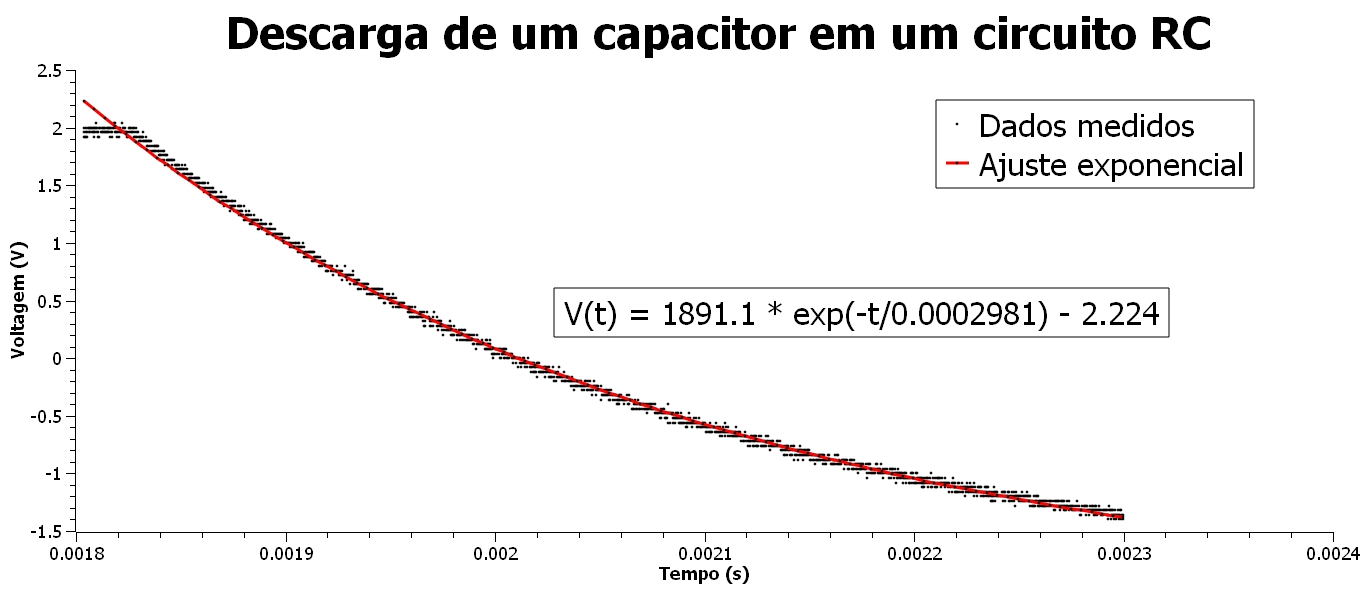
\includegraphics[width=\textwidth]{grafico-lab2.jpeg}
\caption{Gráfico da tensão em função do tempo durante a descarga do capacitor.}
\label{fig:graficos}
\end{figure}

Do ajuste, obtemos os resultados apresentados na Tabela $1$. 

\begin{table}[h]
\centering
\caption{Resultados do ajuste da curva de descarga do capacitor.}
\label{tab:resultados_ajuste}
\begin{tabular}{lcc}
\toprule
\textbf{Parâmetro} & \textbf{Valor} & \textbf{Incerteza (±)} \\
\midrule
Amplitude ($A$) & $1.8911 \times 10^{3}$ & $4.7394 \times 10^{1}$ \\
Tempo próprio ($\tau$) & $2.9810 \times 10^{-4}$ & $1.4730 \times 10^{1}$ \\
Offset ($y_0$) & $-2.2239 \times 10^{0}$ & $9.3733 \times 10^{-3}$ \\
\midrule
\multicolumn{3}{l}{Intervalo do ajuste: $x \in [0.0018036, 0.0022998]$} \\
\multicolumn{3}{l}{Tolerância: 0.0001} \\
\multicolumn{3}{l}{Iterações: 56} \\
\midrule
$\chi^2$ & \multicolumn{2}{r}{$5.0357 \times 10^{0}$} \\
$R^2$ & \multicolumn{2}{r}{$9.9806 \times 10^{-1}$} \\
\bottomrule
\end{tabular}
\end{table}

Dessa forma, verificamos que a equação que descreve a curva de descarga do capacitor no experimento é dada por:
\begin{equation}
    V(t) = 1.8911 \times 10^{3} \cdot (1 - e^{-t/(2.9810 \times 10^{-4})}) - 2.2239 \times 10^{0}
\end{equation}

O valor da constante de tempo do circuito RC é aproximadamente \(298.10 \, \mu\text{s}\), o que concorda com a estimativa que fizemos no laboratório, conforme print do osciloscópio abaixo.

\begin{figure}[H]
\centering
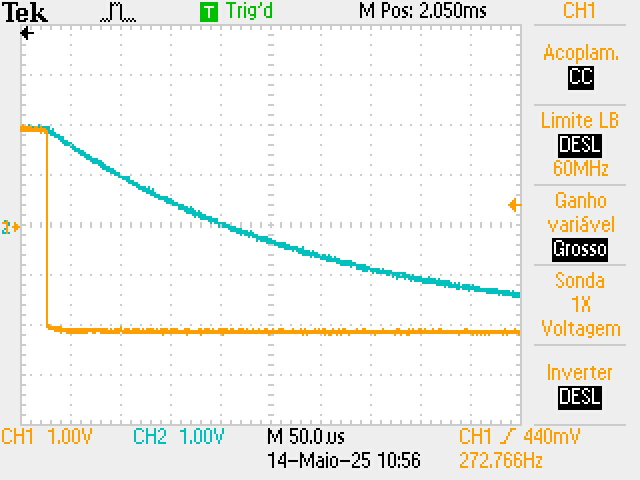
\includegraphics[width=\textwidth]{F0001TEK.JPG}
\caption{Print do osciloscópio mostrando a tensão em função do tempo durante a descarga do capacitor.}
\label{fig:osciloscopio}
\end{figure}

\end{document}